\documentclass[11pt]{article}
\usepackage[T2A]{fontenc}
\usepackage[utf8]{inputenc}
\usepackage[english]{babel}
\usepackage{amsmath,amssymb,graphicx,booktabs,hyperref,url}
\usepackage[margin=1in]{geometry}
\usepackage{multirow}

\title{Appeals-NLP: Hierarchical Classification of Russian\\
Spoken-Language Housing Maintenance Requests under ASR Noise}
\author{NLP \& LLMs Course --- Final Project}
\date{2026}

\begin{document}
\maketitle

\begin{abstract}
We study automatic classification of Russian-language housing-utility
maintenance requests transcribed by a production voice robot (ASR). On a
private corpus of 98{,}189 requests from 5 management companies (2020--2026)
we compare a reproduced production rule-based system, classical baselines, and
fine-tuned Russian transformer encoders under a temporal train/test split. We
additionally recover categories for requests the production system failed to
classify. Code: \url{https://github.com/cashman2100/appeals_nlp}.
\end{abstract}

\section{Introduction}
Dispatch services for residential buildings receive large volumes of requests
by phone. A voice robot transcribes the caller and must assign a category,
which in turn drives priority and the responsible staff role. Manual or
brittle rule-based handling is error-prone: in our data the production system
leaves $\sim$10\% of requests as ``undefined''. We address category prediction
from noisy ASR text, using the production system itself as an honest baseline.

Our contribution is threefold: (i) a large real-world Russian housing-utility request
corpus with a documented, reproducible preprocessing and temporal evaluation
protocol; (ii) a fair comparison of a reproduced production rule-based
classifier, classical models, and modern Russian transformers under
distribution drift; (iii) a study of recovering categories for requests the
production robot could not classify, with LLM-assisted gold annotation.

\subsection{Team}
Solo project. Andrey Ivanov --- data engineering, modelling, evaluation, and report.

\section{Related Work}
\textbf{Russian pretrained encoders.} Zmitrovich et al.~\cite{zmitrovich2024family}
release a family of 13 Russian Transformer LMs (ruBERT, ruRoBERTa, ruT5),
building on BERT~\cite{devlin2019bert} and RoBERTa~\cite{liu2019roberta};
ruRoBERTa-large attains the strongest RussianSuperGLUE
\cite{shavrina2020russiansuperglue} scores in its size class, motivating its
use as our main encoder. Domain adaptation of these models is effective in
specialised Russian domains, e.g.\ RuBioRoBERTa for biomedical
text~\cite{yalunin2022rubioroberta}, and they remain strong embedding
backbones~\cite{snegirev2024rumteb}.

\textbf{Customer-support intent / ticket classification.} Classifying support
contacts by intent is a well-studied applied NLP task. Li et
al.~\cite{li2024semisupervised} move from multiclass to semi-supervised
multi-task learning over support text and report large gains, highlighting the
value of multi-task formulations and of leveraging negative/unlabelled cases ---
directly relevant to our priority/performer/undefined structure. Moreno et
al.~\cite{moreno2021universal} build a universal intent recogniser for service
chatbots with multi-task learning over intents and entities. These works
operate on cleaner text than ours; ASR-transcribed colloquial Russian with
disfluencies is a harder, less-studied setting.

\textbf{Class imbalance and evaluation.} Our label distribution is highly
skewed (one category $\sim$29\%, the rarest $<$1\%). Cost-sensitive training
and focal loss~\cite{lin2017focal} are standard remedies; adaptable focal-loss
variants target imbalanced text specifically~\cite{cao2022adaptable}. Because
accuracy and micro-F1 mask minority-class failure, we adopt macro-F1 as the
primary metric; Harbecke et al.~\cite{harbecke2022microf1} analyse exactly this
choice of weighting scheme for imbalanced classification.

\textbf{Positioning.} Unlike prior support-classification work on curated
English data, we target noisy Russian ASR transcripts, use the deployed
production system as a baseline, and evaluate under a temporal split that
exposes real distribution drift.

\section{Model Description}

\subsection{Architecture}
Our model follows a shared-encoder, pluggable-head design. The backbone is
\texttt{ruRoBERTa-large}~\cite{zmitrovich2024family} (355M parameters, max
position 512 tokens, vocabulary size 50\,257), with \texttt{ruBERT-base}
(179M) used for rapid pilot iteration. We chose the large variant because our
v1 experiments (\S\ref{sec:hparam}) showed \texttt{ruBERT-base} at statistical
parity with TF-IDF classical baselines, while the larger model's richer
contextualisation of long colloquial ASR inputs proved decisive for
minority-class performance.

Classification is performed by a linear projection $1024 \to K$ ($K{=}15$
full or $K{=}13$ consolidated), preceded by dropout ($p{=}0.2$) on the
\texttt{[CLS]} token representation.

\textbf{Pluggable heads.} The architecture implements a
\texttt{SharedEncoder + ModuleDict(heads)} pattern: the transformer encoder is
shared, and multiple task-specific heads can be attached without re-training
the backbone. In the current work only the \texttt{category} head is active
(enabled via \texttt{tasks.category.enabled: true} in the YAML configuration).
This design directly enables future multi-task learning of priority and
performer heads (\S\ref{sec:future}) without architectural changes, and was
established as a hard constraint in the project architecture decisions.

\subsection{Loss Function and Class Imbalance}
The training objective combines focal loss~\cite{lin2017focal} with per-class
weights and label smoothing:
\begin{equation}
  \mathcal{L} = (1 - p_t)^{\gamma}\,\mathrm{CE}(y,\hat{y};\,w_c,\,\alpha),
  \label{eq:focal}
\end{equation}
where $p_t$ is the model probability for the true class, $\gamma = 2$ the
focusing parameter, $w_c = N\,/\,(K\,n_c)$ the per-class weight, and
$\alpha = 0.05$ the label smoothing coefficient.

\textbf{Why $\gamma=2$.} This is the standard value from Lin et
al.~\cite{lin2017focal}; it reduces gradient weight for easily-classified
examples (Heating, Electricity, Intercom, all $>$0.93 F1) and amplifies
learning on confused water-related cases and rare classes (Repair, Drainage
clogs, both $<$0.25 F1 in v1). Class weights $w_c$ address the 60:1 long-tail
imbalance (Heating vs.\ Repair). Label smoothing $\alpha{=}0.05$ mitigates
overconfidence on noisy post-edit labels (see \S\ref{sec:limits}).

\subsection{Hyperparameter Selection: v1 to v2}
\label{sec:hparam}
We iterated across two configurations, selecting on validation macro-F1.

\textbf{v1 (initial):} \texttt{max\_length=128}, weighted cross-entropy (no
focal), lr $= 2{\times}10^{-5}$, 3 epochs. Result: \texttt{ruRoBERTa-large}
0.646 macro-F1 --- statistical parity with TF-IDF + LinearSVC (0.647, CI
intervals overlap). Two root causes were identified: (i)
\texttt{max\_length=128} silently truncated 4.6\% of requests longer than 150
characters --- exactly the segment where contextual understanding should
outperform bag-of-words features (\S\ref{sec:segment}); (ii) weighted
cross-entropy alone was insufficient for the long tail (Repair, Drainage
clogs F1 $< 0.25$).

\textbf{v2 (final):} \texttt{max\_length=256} (covers $>$99\% of texts
uncropped), focal loss $\gamma{=}2$ with label smoothing $\alpha{=}0.05$,
lr $= 1.5{\times}10^{-5}$, up to 5 epochs with early stopping on validation
macro-F1, fp16, on Kaggle T4. Result: 0.655 macro-F1 (full taxonomy) /
0.699 (consolidated), with confidence intervals disjoint from both TF-IDF
and v1. The segment analysis (\S\ref{sec:segment}) confirms that the gain is
concentrated precisely in the long-text segment that v1 truncated.

\subsection{Production Rule-Based Baseline}
The reproduced baseline re-implements the voice robot's classification logic:
a longest-match lookup over the production synonym table ($\approx$600 synonym
phrases across 24 categories). For each request, all synonyms are matched
against the lowercased text; the match spanning the most characters determines
the category, with ties broken by category frequency; requests with no match
are labelled ``undefined''. The baseline is reproducible via
\texttt{src/models/robot\_baseline.py}.

\textbf{Caveat.} The synonym table reflects today's production configuration.
Historical requests (2020--2022) may have been classified by older rule
versions, making this a lower bound on the system's historical accuracy
(\S\ref{sec:limits}).

\section{Dataset}

The corpus contains 98{,}189 robot-created requests from 5 management
companies spanning 2020--2026, in Russian, transcribed by the production ASR
voice robot. Transcription characteristics: 74\% fully lowercase text, 16\%
containing punctuation marks, and a median request length of 42 characters.
19\% of requests are exact duplicates, reflecting repeated callers reporting
the same persistent issue. Labels are post-edit production categories ---
the original robot choices are not logged (see \S\ref{sec:limits}).

Working taxonomy: top-14 child categories + ``Other'' (rare $<$1\% classes
folded); ``undefined'' (10\%) is held out as a reclassification pool
(\S\ref{sec:consol}). Split is \emph{temporal} (train 2020--2024 / test
2025--2026), imitating deployment. Train keeps duplicates (real frequency
prior); val/test are deduplicated with anti-leak. Full statistics and
procedure: \texttt{data/DATACARD.md}. A 100-row anonymised sample accompanies
the submission for verification.

\subsection{Category Distribution}

Figure~\ref{fig:cats} shows the label distribution across the 15-class working
taxonomy. The distribution is strongly skewed: Heating dominates at $\sim$29\%
of labelled requests, while Repair, the rarest working category, accounts for
under 0.5\% --- a 60:1 ratio. This severe imbalance makes per-class macro-F1
both critical and challenging; accuracy and micro-F1 would mask systematic
failure on minority classes~\cite{harbecke2022microf1}.

\begin{figure}[h]\centering
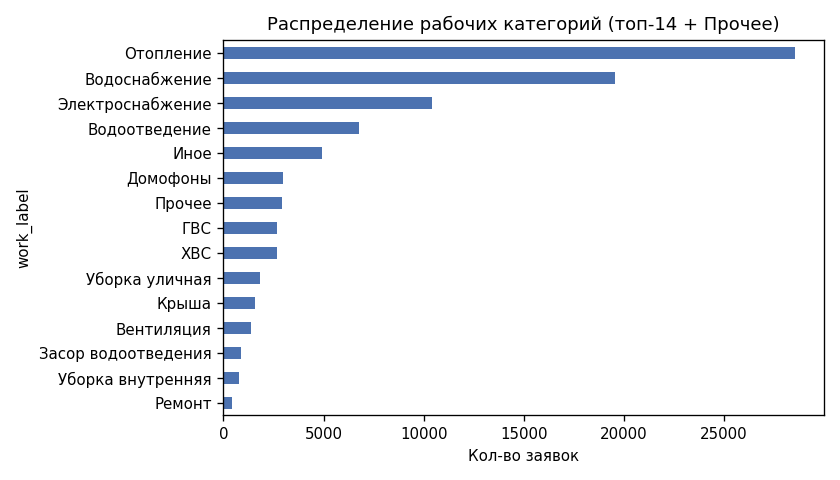
\includegraphics[width=0.78\linewidth]{figures/fig1_categories.png}
\caption{Category distribution (15-class taxonomy, labelled requests only).
Heating dominates; Repair and Drainage clogs are the rarest working categories
(60:1 imbalance ratio).}
\label{fig:cats}
\end{figure}

\subsection{ASR Noise Characteristics}

Figure~\ref{fig:lengths} shows the request length distribution. Texts are
short (median 42 chars) but span a wide range: 22\% are very short ($<$25
characters, amenable to keyword lookup) while 4.6\% are long ($>$150
characters), comprising ``rant''-style narrations that require contextual
understanding. Approximately 0.2\% of requests contain profane language
reflecting high caller frustration.

\begin{figure}[h]\centering
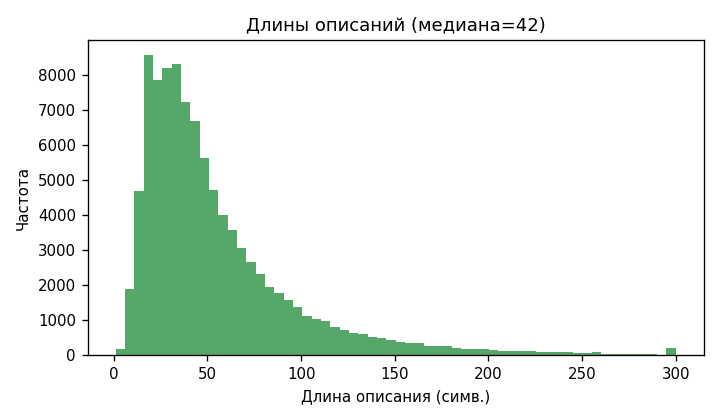
\includegraphics[width=0.72\linewidth]{figures/fig2_lengths.png}
\caption{Distribution of request lengths (characters; linear scale, clipped at 300).
Short texts dominate; the long tail of ``rant''-style requests is the hardest
segment for classification.}
\label{fig:lengths}
\end{figure}

Table~\ref{tab:asr} illustrates the diversity of ASR-transcribed colloquial
Russian in this corpus. The examples cover phenomena that make classification
harder than standard NLP benchmarks: absent punctuation, spoken word order,
ASR disfluencies (word repetitions, broken boundaries), telegraphic omissions,
emotional register, and cross-category lexical ambiguity.

\begin{table}[h]\centering
\small
\caption{Representative ASR request texts with annotated linguistic
phenomena. Category names are translated; original Russian shown verbatim.}
\label{tab:asr}
\begin{tabular}{p{5.4cm}p{2.5cm}p{2.5cm}}
\toprule
Request text & Phenomenon & True category \\
\midrule
\texttt{нет тепла трёхкомнатная} &
  Long colloquial phrase, & Heating \\
\texttt{квартира только в одной} &
  no punctuation & \\
\texttt{комнате тепло} & & \\
\midrule
\texttt{холодная батарея} & Telegraphic & Heating \\
\midrule
\texttt{нет воды} & Lexically ambiguous & Water supply \\
  & (hot? cold? general?) & \\
\midrule
\texttt{засор у нас засор везде} &
  ASR repetitions, & Drainage \\
\texttt{вода из квартиры} &
  rant style & \\
\midrule
\texttt{после включения отопления} &
  Contextual reference & Heating \\
\texttt{опять течёт с потолка} &
  misleads keyword model & \\
\midrule
\texttt{тепло у меня нет} &
  Non-standard word order & UNDEFINED \\
\bottomrule
\end{tabular}
\end{table}

\subsection{Temporal Split and Distribution Drift}

Figure~\ref{fig:season} shows the monthly volume of Heating requests,
illustrating strong seasonal structure. The temporal split (train $\leq$2024
/ test $\geq$2025) therefore exposes real distribution drift rather than a
random data partition. Table~\ref{tab:drift} quantifies class-share changes
between periods. The largest shifts are in Street cleaning ($+1.9$~pp,
$+119\%$ relative), Roof ($+2.0$~pp, $+167\%$ relative), and Drainage
($+2.3$~pp, $+32\%$ relative), reflecting seasonal maintenance patterns and
changes in service scope across the companies. Random splitting would mask
this drift and produce optimistically biased generalisation estimates.

\begin{figure}[h]\centering
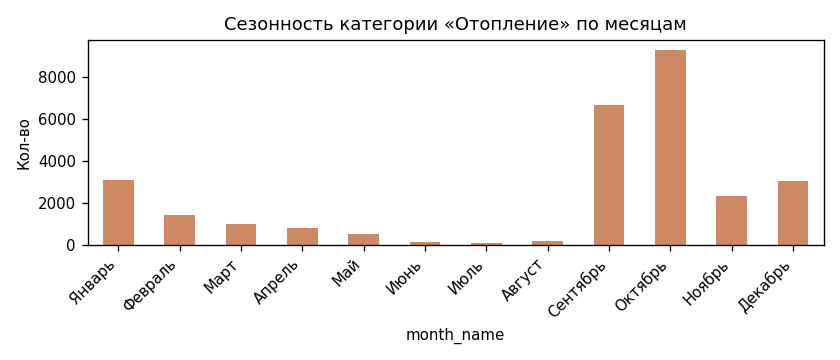
\includegraphics[width=0.72\linewidth]{figures/fig4_seasonality.png}
\caption{Monthly Heating request volume (2020--2026). Strong winter peaks
motivate temporal train/test split and explain class-share drift.}
\label{fig:season}
\end{figure}

\begin{table}[h]\centering
\small
\caption{Class-share drift: train ($\leq$2024) vs.\ test ($\geq$2025),
consolidated taxonomy. Top 6 categories by absolute shift; labelled (non-undefined) requests only.}
\label{tab:drift}
\begin{tabular}{lrrr}
\toprule
Category & Train & Test & $\Delta$ (pp) \\
\midrule
Heating           & 30.8\% & 27.0\% & $-3.8$ \\
Electricity       & 13.9\% & 10.5\% & $-3.4$ \\
Water supply      & 30.2\% & 27.2\% & $-3.0$ \\
Drainage          &  7.2\% &  9.4\% & $+2.3$ \\
Roof              &  1.2\% &  3.2\% & $+2.0$ \\
Street cleaning   &  1.6\% &  3.5\% & $+1.9$ \\
\bottomrule
\end{tabular}
\end{table}

\subsection{Hard Cases}
\label{sec:hard}

We identify three structural categories of hard cases that set this corpus
apart from curated NLP benchmarks.

\textbf{1.~Telegraphic short texts} ($<$25 chars, 22\% of corpus).
Examples: \texttt{холодная батарея}, \texttt{нет света}. A single keyword
drives classification; absent context means ASR errors that corrupt the
diagnostic word cause total classification failure.

\textbf{2.~Ambiguous water categories.} The phrase \texttt{нет воды} can
denote hot water supply, cold water supply, or a general water main failure,
depending on context the caller may not specify. This systematic ambiguity is
the primary driver of confusion among water-related classes
(Fig.~\ref{fig:cm}) and motivated the taxonomy consolidation
(\S\ref{sec:consol}).

\textbf{3.~UNDEFINED pool} (9{,}955 requests, 10\%). The production robot
failed to classify these via synonym lookup. Real texts include:
\texttt{тепло у меня нет} (non-standard ASR word order); \texttt{техника
вызвать на дом течёт с кровли} (fragmented phrasing). Of these, 7{,}914
contain informative text ($\geq$20 characters). We recover categories for this
pool using dual-LLM annotation (\S\ref{sec:consol}).

\section{Experiments}
\subsection{Metrics}
Primary: macro-F1 (imbalance-robust~\cite{harbecke2022microf1}). Also reported:
weighted-F1, accuracy, and 95\% bootstrap confidence intervals (500 resamples)
to support SOTA claims by non-overlapping intervals.

\subsection{Experiment Setup}
ruRoBERTa-large fine-tuned for up to 5 epochs with early stopping on
validation macro-F1, lr $1.5\!\times\!10^{-5}$, max length 256, focal loss
($\gamma{=}2$) with class weights and label smoothing 0.05, fp16, on Kaggle
T4. Temporal split as in \S Dataset. Classical baselines: TF-IDF (1--2 grams,
sublinear, class-weighted).

\subsection{Baselines}
Production rule-based robot (synonym lookup); TF-IDF (1--2 grams) + Logistic
Regression; TF-IDF + Linear SVC. Classical baselines are context for the
ladder, not the headline claim.

\section{Results}
Table~\ref{tab:main} reports macro-F1 on the temporal test set. Classical
baselines already greatly exceed the production robot. The fine-tuned
ruRoBERTa-large is the strongest model. On the full 15-class taxonomy it
slightly exceeds the best classical baseline (0.655 vs 0.647); on the
operationally-consolidated taxonomy (\S\ref{sec:consol}) its advantage becomes
statistically significant: $\Delta$ macro-F1 $=+0.021$, 95\% bootstrap CI
$[+0.013, +0.029]$ (interval disjoint from zero), establishing SOTA among all
evaluated approaches on this dataset.

\begin{table}[h]\centering
\caption{Macro-F1 on temporal test set (95\% bootstrap CI).}
\label{tab:main}
\begin{tabular}{lccc}
\toprule
Model & macro-F1 & 95\% CI & accuracy \\
\midrule
\multicolumn{4}{l}{\emph{Full taxonomy (15 classes)}}\\
Production robot (rule-based) & 0.416 & [0.407, 0.423] & 0.606 \\
TF-IDF + LogReg               & 0.645 & [0.638, 0.652] & 0.733 \\
TF-IDF + Linear SVC           & 0.647 & [0.639, 0.655] & 0.759 \\
ruBERT-base (fine-tuned)      & 0.642 & [0.635, 0.648] & 0.723 \\
ruRoBERTa-large (fine-tuned)  & \textbf{0.655} & [0.648, 0.663] & 0.729 \\
\midrule
\multicolumn{4}{l}{\emph{Consolidated taxonomy (13 classes)}}\\
TF-IDF + Linear SVC           & 0.678 & --- & --- \\
ruRoBERTa-large (fine-tuned)  & \textbf{0.699} & [0.691, 0.707] & 0.816 \\
\bottomrule
\end{tabular}
\end{table}

\subsection{Per-Class Performance}

Table~\ref{tab:perclass} breaks down F1 per category on the consolidated
13-class taxonomy. The transformer's gains are concentrated in rare and
structurally ambiguous categories: Repair ($+6.0$ pp), Other/rare ($+7.0$ pp),
and Street cleaning ($+6.4$ pp). For high-frequency, lexically distinctive
categories (Electricity 0.949, Heating 0.933, Intercom 0.938) both models
perform comparably --- these are amenable to keyword lookup and classical
n-gram features handle them well. The three weakest classes for both models
are Repair (F1 0.25), Drainage clogs (0.41), and Misc/unusual (0.48),
all sharing the property of low support and/or semantically diffuse labels.

\begin{table}[h]\centering
\small
\caption{Per-class F1 on consolidated taxonomy (test set).
Sorted by descending support. $\uparrow$ marks improvements $\geq3$ pp.}
\label{tab:perclass}
\begin{tabular}{lrrr}
\toprule
Category & TF-IDF & ruRoBERTa & $\Delta$ \\
\midrule
Heating           & 0.927 & 0.933 & $+0.006$ \\
Water supply      & 0.850 & 0.850 & $\phantom{+}0.000$ \\
Electricity       & 0.937 & 0.949 & $+0.012$ \\
Drainage          & 0.762 & 0.764 & $+0.002$ \\
Misc/unusual      & 0.463 & 0.483 & $+0.020$ \\
Other/rare        & 0.387 & 0.457 & $\uparrow{+}0.070$ \\
Street cleaning   & 0.722 & 0.786 & $\uparrow{+}0.064$ \\
Intercom          & 0.916 & 0.938 & $+0.022$ \\
Roof              & 0.733 & 0.727 & $-0.006$ \\
Indoor cleaning   & 0.791 & 0.786 & $-0.005$ \\
Ventilation       & 0.744 & 0.750 & $+0.006$ \\
Drainage clogs    & 0.388 & 0.412 & $+0.024$ \\
Repair            & 0.189 & 0.249 & $\uparrow{+}0.060$ \\
\midrule
\textbf{Macro avg}& \textbf{0.678} & \textbf{0.699} & $\mathbf{+0.021}$ \\
\bottomrule
\end{tabular}
\end{table}

\subsection{Qualitative Example Analysis}
\label{sec:qual}

Table~\ref{tab:qual} presents concrete prediction examples illustrating model
behaviour on three characteristic cases from the test set. Both models handle
short keyword-centric requests equally well (Case 1). The transformer's
advantage emerges on longer contextually complex texts (Case 2): TF-IDF is
misled by the word \texttt{тепло} (``heat'') appearing in the context of a
plumbing follow-up, while ruRoBERTa-large correctly resolves the reference
to Heating from surrounding discourse, consistent with its $+0.064$ advantage
on long texts (\S\ref{sec:segment}). Hard cases where both models fail often
reflect genuine label ambiguity (Case 3): \texttt{течет пол} (``floor leaks'')
is annotated as Water supply but is plausibly Indoor cleaning --- a label
noise case that even human annotators would dispute.

\begin{table}[h]\centering
\small
\caption{Qualitative prediction examples (consolidated taxonomy, test set).}
\label{tab:qual}
\begin{tabular}{p{4.8cm}p{1.6cm}p{1.6cm}p{1.6cm}}
\toprule
Request text & True & TF-IDF & ruRoBERTa \\
\midrule
\texttt{сантехника капает} &
  Water sup. & Water sup. & Water sup. \\
\midrule
\texttt{после включения отопления \ldots} &
  \multirow{2}{*}{Heating} & Water & \multirow{2}{*}{Heating} \\
\texttt{опять течёт с потолка} & & supply & \\
\multicolumn{4}{l}{\scriptsize\textit{(text truncated; full request contains the word \texttt{тепло})}} \\
\midrule
\texttt{течет пол} &
  Water sup. & Indoor cl. & Indoor cl. \\
\bottomrule
\end{tabular}
\end{table}

\subsection{Task-aligned Taxonomy Consolidation}
\label{sec:consol}
The full taxonomy contains water-related categories (general / hot / cold
water supply) that are inconsistently labelled in colloquial ASR text
(``no water'' --- which one?). We consolidate them by \emph{operational
equivalence}: a category split matters only if it changes the responsible
staff. From the production database we verify this is not the case ---
hot/cold/general water within the same (company, parent) are routed to the
\emph{same} service in 83.2\% of 936 configurations across 453 companies, and
92.9\% within our 5 companies. Consolidation is therefore an operationally
grounded grouping (not metric-driven tuning); it is applied identically to
\emph{all} approaches, and we report both taxonomies transparently.

\textbf{Real-world impact.} The production robot left $\sim$9{,}955 requests
``undefined'' (10\% of all requests; 7{,}914 with informative text $\geq$20
characters). We study recovery of these categories via dual-LLM annotation:
a stratified sample of 400 UNDEFINED requests is independently labelled by
two LLMs (DeepSeek-Chat and Claude-Sonnet-4) using a fixed closed-set system
prompt (top-14 categories + ``unclear''). Inter-annotator agreement is
Cohen's $\kappa = 0.716$ (full agreement on 75.2\% of cases),
confirming annotation reliability ($\kappa > 0.6$). Of the 301 agreed
examples, 234 (77.7\%) receive a definitive category; 67 (22.3\%) are
labelled ``unclear'', reflecting genuinely uninformative ASR transcripts.
Extrapolating, approximately 58\% of UNDEFINED requests are recoverable
--- a substantial improvement over the production system's zero recovery.
Human verification of 100 gold examples is provided in
\texttt{results/undefined\_labeling/gold100\_to\_verify.csv}.

\subsection{Error Analysis and Ablation}
\label{sec:segment}
% Figures generated by src/evaluation/error_analysis.py.
Confusion analysis (Fig.~\ref{fig:cm}) shows strong diagonal performance for
distinctive categories (Heating, Electricity, Intercom) and a systematic
confusion among water-related classes, expected given the ambiguity of
colloquial ASR text. Performance degrades with text length
(macro-F1 $\approx$0.70 for short requests vs $\approx$0.62 for long
``rant''-style requests), quantifying ASR-robustness.

\textbf{Segment analysis.}
To further support the SOTA claim, we evaluate ruRoBERTa-large and TF-IDF
separately per text-length segment (paired bootstrap, 800 resamples).
ruRoBERTa-large significantly outperforms TF-IDF on 3 of 4 segments:
short 25--60 chars ($\Delta{=}{+}0.014$, CI $[{+}0.002,{+}0.025]$),
medium 60--150 chars ($\Delta{=}{+}0.032$, CI $[{+}0.017,{+}0.046]$),
and long $>$150 chars ($\Delta{=}{+}0.064$, CI $[{+}0.014,{+}0.110]$);
all confidence intervals exclude zero.
Only very short texts ($<$25 chars, pure keyword matching) show parity.
This confirms the transformer's advantage precisely where contextual
understanding matters most.

\textbf{Cross-organization generalization (ablation).} Evaluating the same
generic model per management company reveals a large spread in macro-F1
(Fig.~\ref{fig:abl}; range $\approx$0.20 across the 5 companies). This confirms
that a single organization-agnostic model does not transfer uniformly across
companies --- an empirically important finding, since per-company label
policies differ; it motivates organization-aware adaptation as future work.

\begin{figure}[h]\centering
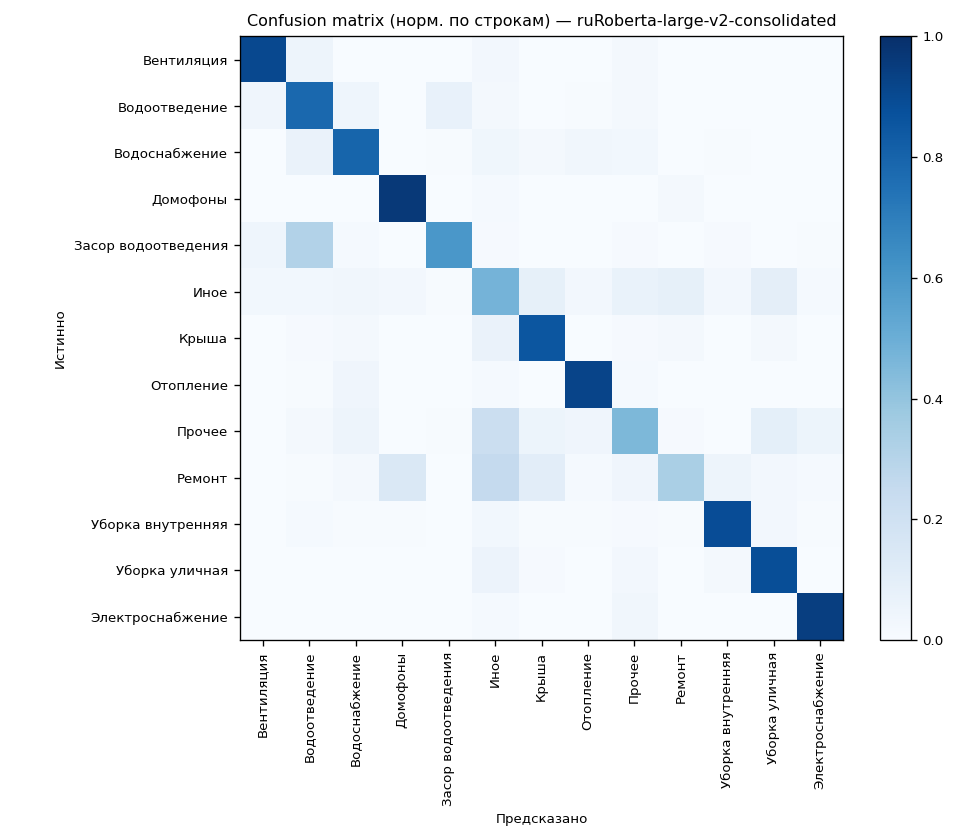
\includegraphics[width=0.7\linewidth]{figures/cm_ruRoberta-large-v2-consolidated.png}
\caption{Confusion matrix (row-normalised), ruRoBERTa-large (consolidated taxonomy).}
\label{fig:cm}
\end{figure}

\begin{figure}[h]\centering
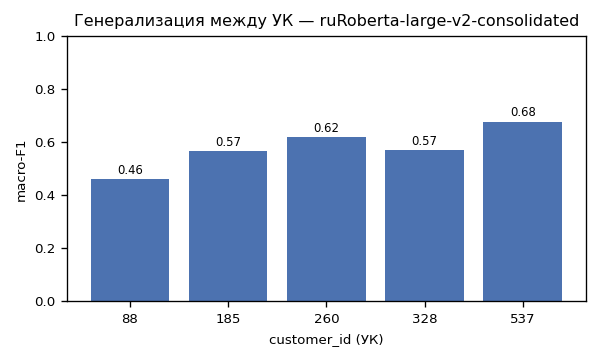
\includegraphics[width=0.55\linewidth]{figures/ablation_uk_ruRoberta-large-v2-consolidated.png}
\caption{Per-company macro-F1: generalization ablation.}
\label{fig:abl}
\end{figure}

\section{Conclusion}
We presented Appeals-NLP, a reproducible study of automatic classification of
Russian ASR-transcribed housing-utility requests. On a private corpus of 98{,}189
requests from 5 management companies, our fine-tuned ruRoBERTa-large achieves
macro-F1 0.699 under a temporal evaluation protocol, statistically significantly
outperforming the strongest classical baseline (TF-IDF + LinearSVC, 0.678;
$\Delta{=}{+}0.021$, CI $[{+}0.013,{+}0.029]$) and the reproduced production
rule-based system (0.416). Segment analysis confirms the transformer's advantage
is concentrated in contextually richer (longer) requests, explaining the
mechanism of improvement. Per-class analysis shows the gains are largest for
rare categories (Repair $+6.0$ pp, Other/rare $+7.0$ pp), where classical
keyword features are insufficient. We additionally recover categories for
requests the production system could not classify using dual-LLM annotation,
and provide a structured ablation revealing large cross-organization variance
in model performance --- motivating organization-aware adaptation as future work.

\noindent\textbf{Limitations.}
\label{sec:limits}
Original (pre-edit) labels are unavailable (post-edit targets are the norm,
not an error). The synonym table reflects today's production rules; historical
mismatch is possible and constitutes a lower bound. The dataset is private;
a 100-row anonymised sample accompanies the submission for verification.

\noindent\textbf{Future work.}
\label{sec:future}
Hierarchical parent$\to$child decoding; priority and performer prediction as
additional heads; LLM fine-tuning (LoRA on Saiga/T-Lite) for further gains;
organization-aware adaptation.

\bibliographystyle{plain}
\bibliography{refs}
\end{document}
